Suppose that a process is currently operating at 3.5 sigma level of quality, and it is planned  to  use  projects  to  move  this  process  to  a  6 sigma  level.  What  project improvement rate would be necessary to achieve that new performance in 2 years? 
        
    \begin{figure}[h]
        \centering
        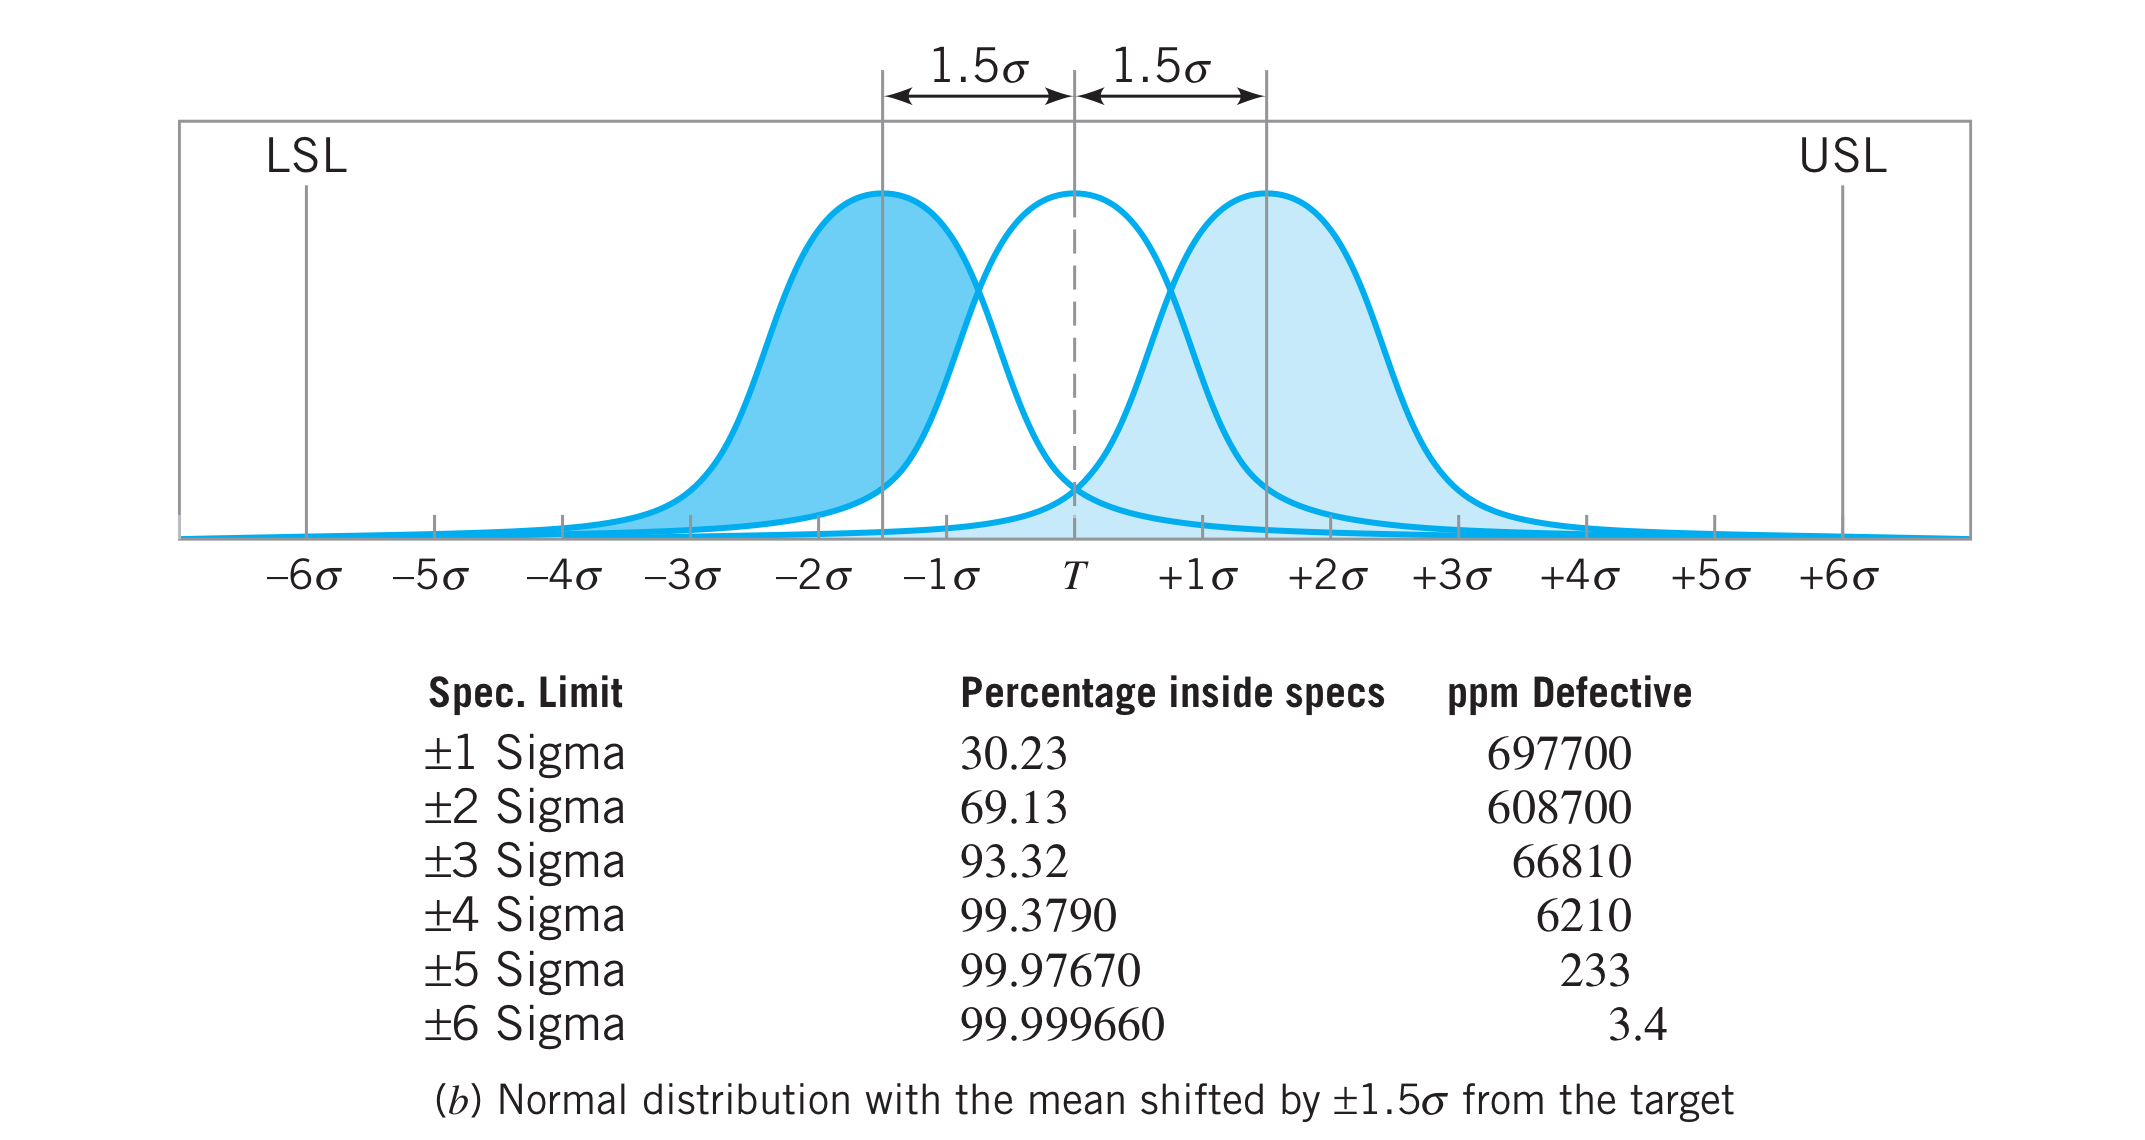
\includegraphics[width=8cm, height=5cm]{figures/normal distribution.jpeg}
        \caption{normal distribution}
        \label{fig:1}
    \end{figure}
 
    \begin{align*}
        & (\text{NORM.S.DIST}(-1, \text{TRUE})) \times 1000000 = 158655.2539 \\
        & (\text{1-NORM.S.DIST}(5, \text{TRUE})) \times 1000000 = 0.286651572 \\
        & 3.4 = 158656 \times (1-x)^2 \\
        & 3.4 / 158656 = (1-x)^2 \\
        & ln(3.4 / 158656) = 2ln(1-x) \\
        & 2 = ln(3.4 / 158656) / ln(1-x) \\
        & \text{Thus, the improvement rate} = x = 0.99537 \approx 0.9954 \\
    \end{align*}